\documentclass[12pt]{article}
\usepackage[top=1in, bottom=1in, left=1in, right=1in]{geometry}

\usepackage{setspace}
\onehalfspacing

\usepackage{amssymb}
%% The amsthm package provides extended theorem environments
\usepackage{amsthm}
\usepackage{epsfig}
\usepackage{times}
\renewcommand{\ttdefault}{cmtt}
\usepackage{amsmath}
\usepackage{graphicx} % for graphics files
\usepackage{tabu}

% Draw figures yourself
\usepackage{tikz} 

% writing elements
\usepackage{mhchem}

% The float package HAS to load before hyperref
\usepackage{float} % for psuedocode formatting
\usepackage{xspace}

% from Denovo Methods Manual
\usepackage{mathrsfs}
\usepackage[mathcal]{euscript}
\usepackage{color}
\usepackage{array}

\usepackage[pdftex]{hyperref}
\usepackage[parfill]{parskip}

% math syntax
\newcommand{\nth}{n\ensuremath{^{\text{th}}} }
\newcommand{\ve}[1]{\ensuremath{\mathbf{#1}}}
\newcommand{\Macro}{\ensuremath{\Sigma}}
\newcommand{\rvec}{\ensuremath{\vec{r}}}
\newcommand{\vecr}{\ensuremath{\vec{r}}}
\newcommand{\omvec}{\ensuremath{\hat{\Omega}}}
\newcommand{\vOmega}{\ensuremath{\hat{\Omega}}}
\newcommand{\sigs}{\ensuremath{\Sigma_s(\rvec,E'\rightarrow E,\omvec'\rightarrow\omvec)}}
\newcommand{\el}{\ensuremath{\ell}}
\newcommand{\sigso}{\ensuremath{\Sigma_{s,0}}}
\newcommand{\sigsi}{\ensuremath{\Sigma_{s,1}}}
%---------------------------------------------------------------------------
%---------------------------------------------------------------------------
\begin{document}
\begin{center}
{\bf NE 250, F15\\
October 21, 2015 
}
\end{center}

\textbf{Monte Carlo} for neutral particle transport

So far we've talked about the diffusion equation, derived the transport equation a few ways, and talked about the adjoint. \\
I'd like to spend the next bit of time talking about Monte Carlo methods, variance reduction, and how we can use the adjoint with variance reduction (note that I've totally just canned the syllabus). \\
After that we'll move into discretization and solution methods for the deterministic transport equation. 

What is Monte Carlo?
  \begin{itemize}
  \item The use of \textit{random processes} to determine a \textit{statistically-expected} solution to a problem
  \item Random processes can fulfill two roles:
  \begin{itemize}
    \item Statistical approximation to \textit{mathematical equations}
    \item Statistical approximations to \textit{physical processes}
  \end{itemize}   
  \item Construct a random process for a problem, 
  \item Carry out a numerical simulation by N-fold sampling from a (pseudo-)random \# sequence
\end{itemize}

For MC in radiation transport, we simulate many independent particles in a system:
\begin{itemize}
\item Treat each physical process as a \textit{probabilistic process}
\item \textit{Randomly sample} each process using an independent stream of pseudo-random numbers
\item Follow each particle from birth until it no longer matters
\item Accumulate the contributions of each particle to find the statistically-expected mean behavior and variance
\end{itemize}

\textbf{WHY?}\\
Monte Carlo, when done properly, can be highly accurate and can be considered a ``gold standard" answer. Table~\ref{tab:comparison} compares MC and deterministic methods.
%
\begin{table}
\begin{center}
\begin{tabu}{| X | X |}
\hline
Monte Carlo         & Deterministic \\\hline
% -----------------------
* General geometry    & * Discretized geometry \\
* Continuous Energy   & * Multigroup in energy\\
* Continuous in Angle & * Angular Quadrature\\
* Number of particles governs solution accuracy & * Variable discretization governs solution quality \\
* Must adequately sample phase space & * Must adequately discretize phase space \\
* Solutions have statistical error & * Solution contains truncation error\\
* Local solutions only of variable quality & * Global solutions of equal quality \\\hline
% -----------------------
* Easy to parallelize on CPUs & * Can be complicated to parallelize on CPUs\\
* Slow & * Can be quite fast \\
* Might be memory intensive & * Might be memory intensive \\
* Need efficient Variance Reduction & * Need acceleration methods \\\hline
  \end{tabu}
  \caption{Comparison of Monte Carlo and Deterministic Methods}
  \label{tab:comparison}
\end{center}
\end{table}

\begin{figure}[h!]
\begin{center}
  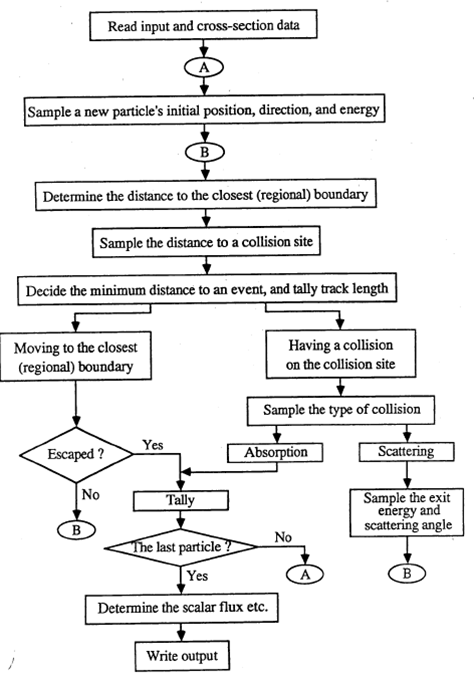
\includegraphics[height=6 in,clip]{../figs/MC-algorithm}
\end{center}
  \caption{Monte Carlo neutral particle transport algorithm}
  \label{fig:mc-algo}
\end{figure}
%
Figure~\ref{fig:mc-algo} shows the algorithm that is basically what happens in MC. 

General purpose MC codes in nuclear:
\begin{itemize}
\item \textbf{MCNP}: developed at LANL, distributed via RSICC, \href{http://rsicc.ornl.gov}{http://rsicc.ornl.gov}
\item \textbf{Geant4}: developed by a large collaboration in the HEP community, \href{ http://geant4.web.cern.ch/geant4/}{http://geant4.web.cern.ch/geant4/}
\item \textbf{EGSnrc}: developed at NRC (Canada), \href{http://www.irs.inms.nrc.ca/EGSnrc/EGSnrc.html}{http://www.irs.inms.nrc.ca/EGSnrc/EGSnrc.html}
\item \textbf{SERPENT}: Developed by Dr. Jaakko Leppanen, VTT, Finland, \href{ http://montecarlo.vtt.fi/}{http://montecarlo.vtt.fi/}
\item \textbf{Shift}: developed at ORNL, distributed via RSICC, \href{http://rsicc.ornl.gov}{http://rsicc.ornl.gov}
\end{itemize}


\end{document}
